\chapter{迷雾}

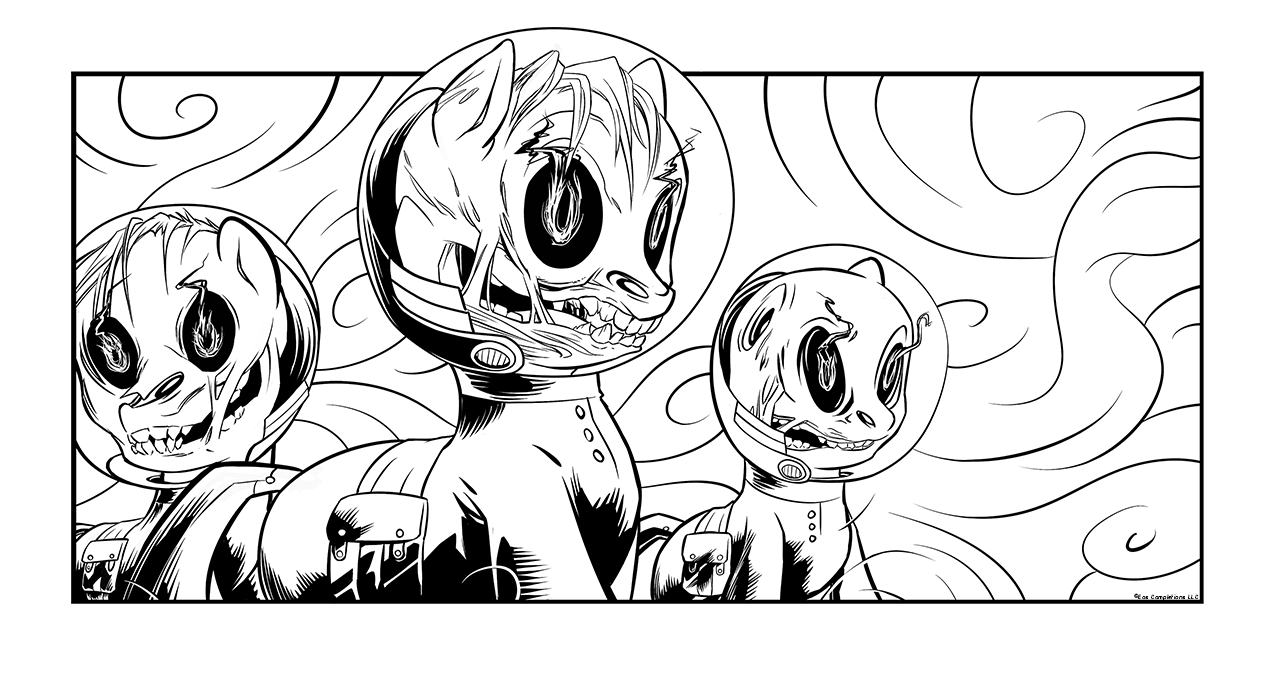
\includegraphics[width=0.9\linewidth]{image18.png}

\begin{intro}
    为熊孩子带来的浩劫而哭泣吧!\footnote{这一句话恶搞莎士比亚的凯撒大帝}
\end{intro}

\daytimeplace{14}{6:00 AM}{纪念碑镇,52号国道南段}{The Memorial, Big 52 S Branch}

「哦咿呦……」

白先生走进窝棚,低头看着长耳坐在一圈小骨头围成的一个圆环之中,她的角上挂着很多发亮的小珠,看起来就像一蘸提灯。雌驹用一个奇怪的姿势坐着,她的后蹄子盘在身体前面,前蹄像绽放的花朵一样打开。她真是……太奇怪了。这个先知居然不是一个斑马。公马对此非常好奇。

在房间的另一边,灌木正在为去铁砧镇而做着最后的准备,白先生的侄子完全不受长耳的影响,仔细地整备着他的武器。

「好吧,她到底在干啥?」白苹果的领袖一脸迷糊地看着那先知。

灌木耸耸肩,「我不清楚,她说她要作法让敌人笼罩在什么『战争迷雾』之中,然后就嗑了一大堆药坐在那里『哦呦哦呦』到现在。」

「嗑药?」白苹果皱了皱眉头,整个屋子里面都是药草燃烧的味道,熏得他晕晕乎乎的。那些气味很奇怪,虽然觉得不对头,不过他也说不上来哪里不对。

「哦呦呵……」

「比如说,曼他特啥的,吃了超级多,还有很多白色的药片和从来没有见过的绿色东西,她把一部分放烟壶里面抽了,然后把剩下的灌肚子里……而且她还喝了不少,你懂的,对于我的酒量而言,不少是多少。」

「然后呢,她就那样神神叨叨的?」

老白觉得自己眼前也开始出现点点了,就像鬼火一样,让他觉得有些朦胧,屋子中间的熏香味道实在太浓,让他觉得眼前的一切就好像是做梦一样。

公马摇了摇头,不,不是做梦,是因为那些药品,那些药品切断独角兽对于现实的感知,让小马能专注于魔力的流动,不过那种东西非常非常容易上瘾,而且有毒。

「你说到什么雾?」

灌木点点头,「没错,她叨叨着什么『战争迷雾』之类的,然后就不说话了。」

白色的独角兽抚摸着自己的下巴思索着。「『战争迷雾』?那是啥,把云丢到敌人脑袋上?」老白一点都不明白。

「马上就知道了。」狙击手已经打包好武器,他看起来完全不受那些烟雾影响,或许是因为他的身体比较强壮。「不过如果她不赶快醒来的话,我们只好把她丢在这里了……我还是挺想念她。」

老独角兽皱起眉头,「你可别低估了她,说不定她还能救你一命!」不管谁都可以看得出来那个独角兽老太太不一般,不过,老白也知道和他侄子说那种事情是浪费时间。

「哦咿呦……」

灌木嗤之以鼻:「怎么救,预言我今天会挨几颗枪子?」

和他解释果然是浪费时间。

「或者说,替你挡一两颗枪子?」老白叹了口气。「我们走吧,这里味道臭死了。」

\horizonline

\daytimeplace{14}{6:30 AM}{铁砧镇,52号国道南段}{Ironworks, Big 52 S Branch}

「这位就是那个传闻中的小幽灵?」有着红色鬃毛的红色独角兽低头看着帕比,「一点都不起眼嘛。」

砍刀讪笑着,「马不可貌相,这小家伙简直不可阻挡,而且还会修理各种电子设备。」不过红色公马看起来完全没什么兴趣。

「随便,你想要个宠物的话,怎么都好。赶紧干活去,要不你拿工具去下面帮那些家伙弄开避难厩大门。」

「小菜一碟。」砍刀走回他的部下面前,「你们也听到了,我们去撬开那核桃然后拿财宝去!」他拍了一下帕比的屁股说:「你也一起下去,小幽灵。」

帕比现在很不开心,因为她刚刚又被训斥又挨了打,虽然打屁股现在一点都不疼,但是她觉得心里非常非常疼。因为平常妈妈虽然也训斥她,有时候也打她屁股。但是如果帕比说她知道错了妈妈马上就会抱着她安慰她。这些小马则只是在一边站着嘲笑她,让她觉得很伤心,也没有谁来抱她告诉她没关系。她觉得她应该表现得很能干很厉害,然后这些小马才会喜欢她,就像她刚刚修好无线电台的时候那样。

小雌驹的思绪被塑料花打断了,

「嘿磨蹭鬼,你来还是不来?」

「当然,我来……」帕比有气无力地回答着,然后小雌驹立刻屁颠屁颠地跟着那几匹马走过去了。

血浴看着这群小马走开,然后低头看着桌子上的地图,视线从铁砧镇的红圈上跳到52国道上一个又一个小镇上。他露出一阵满足的冷笑,探子回报纪念碑镇已经完全被遗弃,那么接下来就变得更简单了。

现在这个强盗头头心中的唯一芥蒂就是来自北边的小麻烦,好运的坦克完全失去联络,而那群红蟑螂饭桶也没找到一丝线索,反而带回一个穿着防辐射服的智障儿。

52号国道的幽灵……如果她真的是英雄的话,看起来也没什么威胁,而且更好的是,她现在已经是野牛帮最烂小队的吉祥物了。52号国道的居民应该选个更好的英雄。

一个飘进来的机械精灵打断了血浴统治52国道的美梦,他非常恼怒的瞪着入侵者。

「又咋了?」

机械精灵闪着蓝光发出旭日系统的声音,「血浴,这样不对,用现有装备切开避难厩大门需要花费大量时间,我强烈建议我们继续北上,否则会给敌人组织防御力量的时间。」

血浴笑了起来,「给他们多少时间也没用了!它们不过是等着被打翻的保龄球瓶而已,我们现在在这里以逸待劳,然后让整条52国道都在我们前进的马蹄下颤抖,然后他们就会在恐惧之中拜倒在我蹄下!他们绝对不会反击,他们只会逃跑。就算子弹可以挡得住,但是没有东西可以挡得住恐惧本身。」

旭日系统看起来对这段煽动演说毫不感冒,「洗脑才更加有效率,根据我的计算,你只是在毫无意义地杀戮行为上浪费大量的资源,或许我需要寻求更佳解决方案了。」

公马恼怒地皱着眉头,走到那个机械精灵面前面对着它。「你这个没用的破烂给我听好了,你给我们武器和机器马,但是你要搞清楚,我才是野牛帮的头头,是我给你分享胜利果实的机会。等我们碾碎了52号国道,我可以给你足够的地方和瓶盖让你买奴隶来重建你的什么太阳帝国。但是这些小马,这条52国道上的所有小马,一个活口都不能留,我可不想给他们翻账的机会!」

旭日系统只是静静地等他扯完长篇大论,然后说:「这违背我们当初的合作协定,如果你继续这种行为,我将会撤离所有战斗机甲,或许我该找个更好的合作伙伴了。」

血浴冷笑一声:「你觉得你可以要挟我?我才不在乎你那没用的铁罐,我现在有足够的坦克和重武器!」公马一蹄子把一个空箱子踏得粉碎。

「那好,再见。」机械精灵说着转头飞走。

「等等,肏蛋货……算你赢了!你去楼下告诉那些撬避难厩大门的小马,让他们只杀掉反抗的,剩下的抓做俘虏。」红色独角兽啐了一口低声说,心想,反正我们之后可以随时处决他们。

机械精灵满意地点了点头,「很好,你还是讲理的,那么回头见。」机器说着飞出了帐篷,飞入浓浓的晨雾之中。

在那机器飞出帐篷之后,另一只小马走了进来,「我说老大,这雾气不停地从山上涌下来,就算不是独角兽,也能看出来有谁在给这里施咒……」

血浴大笑着,「那些孬种,他们觉得这种东西可以掩盖他们的驽弱偷袭?别笑掉我的大牙了。」独角兽狂笑了一阵之后,走出了帐篷开始下命令,「所有带哔哔小马的带队出去巡逻,给他们每匹马一把冲锋枪和曼他特。」

那个部下点点头,「马上去办!」他说着跑出了帐篷。

在迷雾之中,三个黄色的小小身影寻觅着帕比的蹄印,慢慢靠近营地。

\horizonline

\daytimeplace{14}{7:30 AM}{铁砧镇,52号国道南段}{Ironworks, Big 52 S Branch}

「肏他妈的王八壳子!」

砍刀泄气地踹了避难厩大圆合金门一蹄子。随着一声坚实的声音回荡在入口的通道中,那公马抱着自己的蹄子哀嚎起来。

\begin{center}
    蹄子 vs 反超聚魔法合金门

    失败
\end{center}

而在避难厩入口的地板上已经堆满了各式各样的工具,而现在红蟑螂小队正在一起用一台等离子切割机对大门下蹄,但是到目前为止,他们唯一创造性的行为就是创造了一连串对圆形大门的新颖咒骂方式,但是却从未穿破那合金门的第三层隔热板。

不过和那些气急败坏尥蹶子的强盗不同,帕比现在玩的很开心。因为那个打屁股老妖婆已经不见了,而这里这么多小马还这么多玩具。她玩儿了半天的捉迷藏,赢到了她能想到的所有捉迷藏奖项。比如说抓鬼大师,躲藏大师,最萌参赛者等等,不过最主要还是没有小马真的会和一个小孩子认真玩,而且小雌驹也很擅长这个游戏。所以为了庆祝她的胜利,她决定和一个电弧焊枪还有几个合金大锤一起开个庆祝茶会。在她玩累之后,她的注意力转向那个大门旁边闪闪发光的控制台。

「为啥你们一直欺负这个门?」小雌驹想闻闻那个等离子切割机冒出的烟,但是头盔却撞上了金属大门。

「为啥不『欺负』大门蠢货!我们要打开它!」

帕比坐了下来,「为啥,你们想和里面的漂漂马做游戏么?」

臭尾大笑起来:「对,差不多就是那样。」

帕比看了看大门,然后又看了看旁边的控制器。这是一个她得到那些小马尊敬的绝佳机会,因为她被打屁股之后那些小马一直把她当傻瓜看。

「嗯哼,或许人家知道怎么打开它。」

房间里面的每一个小马都转头看着快乐帕比。然后砍刀说话了:「你没开玩笑吧?你知道怎么打开这门?」

「那是,超简单!你只要对那个声音说什么『身份别史马』,然后在说什么……嗯,密码,然后这个大门就开啦!」

公马一脸迷糊的歪着头:「呃,你知道密码?」

「那是当然,我当然知道密码,我是谁啊!」帕比摇了摇头,「嗯哼,看我的!」

小雌驹跑到控制台边,然后踮起后蹄,将一只黄色小前蹄按在绿色的按钮上。但是那个控制台只发出了沙沙声。小雌驹有些呆呆地看着控制台说。「呃……不应该这样啊?」

切纸咳嗽一声,「呃,我们曾经对那个东西做了一点点……改造……或许……它现在坏了?」

帕比皱起的眉头变成了微笑,「坏了?别担心!我能修好!」

\horizonline

\daytimeplace{14}{8:00 AM}{铁砧镇,52号国道南段}{Ironworks, Big 52 S Branch}

强盗打着哈欠,盯着视觉增强魔法\footnote{视觉增强魔法(Eyes Forward Sparkle):哔哔小马的功能之一,类似于一个魔法版的雷达}上闪烁的光点。寻找着可能出现的红点,没有,没有,啥也没有……{}

「肏蛋的雾,老娘还想回去继续扒商店里的东西。」

另一个独角兽给了她伙伴脑门上一蹄子。「闭嘴,招子放亮点,看好你的雷达,我可不想因为你丫巡逻走神和你一起死得不明不白。」

「滚边去!」带着哔哔小马的雌驹叹了口气继续看着那浓厚的雾墙,那东西绝对不普通,因为它一直在干扰着敌我识别器,浓雾深处一直有红点和黄点闪来闪去,但是走近看又什么都没有。「这浓雾太诡异了,感觉就像是有什么东西会突然蹦出……」

忽然一个红点出现了,跟着又出现两个,那卫兵一边看着稳定的红点一边举起了步枪,同时轻轻敲着蹄子,另一个卫兵心领神会地举起武器指向她枪口的方向。

那些红点移动得并不是很快,而且并没有什么声音,不过既然红点刚刚出现,那么说明敌人距离他们还有段距离,卫兵聚精会神地举起武器。

啪嗒……{}

两个雌驹瞄准着浓雾深处绷紧了神经。

啪嗒……{}

这里距离营地很远了,只能隐约听到其他强盗打闹吼叫的声音,不过在喧闹声之间,卫兵清晰地听到蹄子踏在地面上的声音。

「开枪啊!快开枪!

哒哒哒哒哒哒!

两把突击步枪喷出火舌,将金属风暴射向敌人应该在的方位,然后在浓雾之中传出一阵尖啸。三个红点消失了,同时步枪也打光了子弹。

「肏他妈那是什么……」卫兵的咒骂被无线电打断了。

「蝴蝶前哨,我听到了你们那边的枪声,发生什么了?」

「有几个蠢货想趁浓雾偷袭我们,不过我们干掉它们了,我们现在去检查那是什么东西。」那个带着哔哔小马的卫兵回话的时候,她的伙伴走进迷雾之中检查红点消失的位置。

「明白,等你们发现什么再呼叫我。」

「我说,你听到了么,坏马芬,去看看那是什么,然后赶紧回来!那东西跑得貌似不快。」

「我说,钉棒,我想我们好像不小心杀了红蟑螂的吉祥物了!」坏马芬的声音听起来没走多远,于是钉棒寻觅着声音慢慢摸过去。

「等等,怎么还有一个那种小孩,发生什么事了?」

「我不知道,把她拖过来我们仔细看看。」钉棒一边说着一边向着她伙伴代表的黄点走过去,不过忽然三个红点出现在黄点旁边,她惊叫起来,「马芬,快回来,那是陷阱!」

「你说啥?咿!放开我啊呀呀呀!」在一声痛苦的尖叫声中,黄点立刻消失了。钉棒连忙举起枪对准红点的方向,包裹着突击步枪的魔法立场剧烈颤抖着,她用力扣下扳机,但是枪唯一发出的声音就是撞针碰到空弹仓清脆的『咔』一声。她这才想起来自己忘记换弹了。

「我肏,肏肏肏肏!」雌驹惊恐万状地低头摆弄着自己的步枪,她刚刚用魔法拿下旧的弹匣,然后一个软软的东西落在了她的脸上,她愣了一下神,然后才反应过来,这个东西是……坏马芬的蹄子……而且这东西完全被怪力扯了下来。

啪嗒……{}

什么东西落在了她的背上,强盗吓得跳起来没命地跑,但是马上她就感觉到有什么东西抱上她的脖子。在惊恐之中她低头看到的是——一对黄色塑料防护服覆盖的小蹄子……还有自己被扯下脑袋之后的身体。

\horizonline

\daytimeplace{14}{8:00 AM}{铁砧镇,52号国道南段}{Ironworks, Big 52 S Branch}

帕比的黄色小屁股在避难厩大门控制面板拆下来之后露出来的洞口外晃来晃去,时不时地还有电线,电路板之类各种零件被丢了出来。她已经这么折腾了快一个小时了,门口的小马开始怀疑这小妮子到底知道不知道她自己在干啥。

「快弄好了!」帕比的情况报告随着一大堆被扯下的零件飞过房间。「我现在只要给这东西再来两蹶子,然后它就和一个茶壶一样了!」

「像个什么一样?」伤管满脸狐疑地走过去,「我不觉得你把这玩意拆成零件能『修好』它。」

「别担心!我看见我妈妈干这种事情很多次了!只要你踢得够用力什么都能修好!真的!」帕比用「命运之石」咣咣咣地敲打着那个控制台面板。

「别看了懒蛋,起来干活!」砍刀发火了,「那门不会自己把自己切开!」

其他小马一边抱怨着一边拿起工具。

帕比从控制台缺口探出她脏兮兮的头盔大叫着:「等等,再给我一次机会,真的!不骗你们!」帕比说着,用力尥起蹶子给了那东西最后一下子。

然后歪在一边的控制台面板亮了起来。

「{\mt 警告!警告!入侵警告!}」

整个大厅都亮起了红灯。

所有强盗惊恐地聚集到房间的中央,屁股对屁股,举起武器相互掩护着。

「{\mt 清洗该区域。}」

地板上打开几个陷阱门,然后露出四个顶端有个大圆球,然后中间有一堆由大到小圆环的奇怪装置,那些圆环之间闪烁着蓝色的电火花。

砍刀对着其中一个装置开枪,但是小口径子弹在那金属装置的表面上弹开了。红蟑螂的领队带着绝望而又愤怒的表情冲向帕比,「你干了什么蠢货,你会害死所有……」

啪滋!

一道明亮的闪电在一秒钟之内横扫过整个房间,等闪电消失之后,房间里只剩下一撮撮冒烟的灰烬,还有一个毫发无伤的帕比。有时候穿着一个蹄子上接地的环境防护服真的很有用。

\horizonline

\daytimeplace{14}{8:30 AM}{铁砧镇,52号国道南段}{Ironworks, Big 52 S Branch}

那永不消散的超自然浓雾让瞭望塔的狙击手根本看不到地面的情况,不过蝴蝶前哨临死前在无线电中的哀嚎让营地里面所有小马都知道有什么不对劲了。因为这样差劲的能见度,整个营地的小马都开始准备肉搏兵器,动力爪,链锯剑,动力蹄甚至还有其它各式各样的武器,所有小马都编队行动确保没有谁落单。整个野牛帮都严阵以待,静候突袭者来临。

可问题在于,进攻者比他们彪悍多了。

绿蝗虫小队在北边不小心踩到了蓝壁虎小队,或者说是踩到了那队武装到牙齿的小马尸体。虽然这些强盗觉得自己已经足够血腥残忍了,但呈现在她们眼前的光景让她们不寒而栗。

一个高大的雄陆马胸口的铠甲看起来只是有个蹄子大的洞,但是那个洞深达他的心脏,而且不知道是什么东西把他的内脏都从那个洞扯了出来丢得到处都是。香蕉树,那位绿蝗虫小队最年轻的成员在想,那个公马在临死之前看着自己的心脏在面前被撕碎的……那雌驹想到这里忍不住吐了出来。

一个穿着战斗鞍的雌驹被像纸片一样扯成两半,她的后腿和屁股被丢到距离身体老远的地方,而她的肠子肚子在这之间像打碎鸡蛋的蛋清一样洒了一地。

矮胖子坐在墙根,那个雌驹绝望地抱着一个空掉的医疗药水瓶,她显然不是立刻死掉的……她还有时间喝下一瓶药水,而且意识到那东西救不了她。

狙击手黑花园喊道:「毒刺,我想我找到其他两个了。」另外两个小马背靠背站着,被一根长矛戳穿,袭击者甚至没有用长矛的尖头,而是用钝头和蛮力将他们俩像烤肉一样穿成了一串。

队长毒刺看着四具死尸说道:「我们最好睁大眼睛,他们绝对会埋伏我们,动作要轻,留神任何声音,不管是谁干出这种事,他的动静肯定不小。」

就在这个时候,在他旁边出现了一个幼驹大小的黄色身影。

\horizonline

\daytimeplace{14}{8:30 AM}{铁砧镇,52号国道南段}{Ironworks, Big 52 S Branch}

「计划有变,你们老大刚下达了命令,你们不准杀死不抵抗的小马,特别是小……你这个小鬼!」

机器精灵飘进了避难厩大门入口,但是他看到的却是个一脸困惑表情的黄色小鬼头,正在玩着一堆灰烬。机械精灵发出的蓝色光芒难以置信地闪了闪,然后又绕了一大圈,最后飞到了帕比面前。「好吧,又是一堆尸体和我的头号克星,018号终端……为啥我一点都不觉得惊讶,这里到底发生什么了?」

帕比停下了对曾经是她队友的那堆灰烬的『急救』,转过头来看着旭日OS,「呃……你好,提问者,为啥你今天声音不一样了?」

「我再说最后一次!我的名字叫做『旭日系统』不是蓝音,或者虫子,或者提问者!旭!日!系!统——旭日系统!一共就四个字,发音也没那么难好么!还有你在这里做什么,为啥你的敌我辨识码现在是野牛帮,为啥……为啥……为啥!除了你以外这里每一个还能正常沟通和交流的小马都变成灰了?」

帕比戳着自己头盔下面,一脸深思熟虑的神情。她琢磨了一下,然后回答道:「呃,说起来好笑,我刚刚正在修那坏掉的门,但是忽然『吧滋!』的一声,我的朋友好像都伤得很重……我很想去找谁来帮忙,但是我不想再被打屁股了,所以……呃……」帕比说着,一边用蹄子捧起那一撮曾经是伤管的灰烬然后继续说:「……所以……我想等他们其中有谁稍微好一点之后让她去找小马下来帮忙。」小雌驹说完之后低下了头,不过片刻后又赶紧抬起头补充道:「真的!我发誓这不是我的错!」

那个机械精灵扫描了其中的一个电磁线圈,吃惊地问:「你……你是怎么在外面启动了防御系统的?这必须是有超级管理员权限的终端才能做到!而且还需要至少四道安全认证,你你你你是怎么做到的?」

蓝先生一下说了太多的问题让帕比都有些迷糊了,「呃……不是我干的!不是我的错!我刚刚一直修得很好,然后忽然就不知道为什么出错了,不过我没看到怎么回事,因为我的头盔给卡到那个洞洞里了!」帕比指着那个被拆坏歪到一边的控制面板。

旭日系统飞到了控制板旁边,那个机械精灵哔哔哔地发出一阵滑稽的电子音,「你……你你你……你居然把所有避难厩的控制权限全弄到这一个面板里面了?这、这绝对会烧毁避难厩电脑主机的!你这个怪物!又一次毁掉了废土上的一个无价之宝!」

帕比歪着头,一脸迷茫地看着机械精灵:「哦哦哦,我可以得到点心做奖赏么?」

这个自律智能没有回答,他有成吨的脏话要吼给这个小鬼头,但是这个小雌驹绝对是完全听不懂,而且还开心地叫着「耶,点心!」之类地蹦来跳去,这么做简直是浪费时间。

「不能!你的脑子是不是全都变成粉雾了?」

「粉?哦哦哦,我想起来了!声音小姐!你们相亲相爱了吗?」

「谁?P7?」旭日系统完全被这个问题问傻了,现在这状况她问这个问题是想做啥?「没,好吧……或许是?我不清楚。」

帕比一言不发地歪着脑袋,等机械精灵继续说。

「我们相互联系了大概十几次,我们觉得我们之间有很大的……差异。我都不知道她的计算回路到底是怎么搭建的,但她不管做什么都看起来非常有效率,她的程序里面没有写入任何军事用途代码实在是太可惜了。所以她一点用都没有。」

小雌驹笑了起来,在这段分析之后加上自己的结论。

「但是她很可爱!」

「可爱?」

「你懂的,你有没有想要抱抱谁的那种感觉,那就是可爱,比如说……我就很可爱!」帕比露出一副天真的微笑。

「抱抱?」

「好吧,不一定是抱抱……不如说……你在想一个可爱的东西时,你想要一直陪着她,给她做很多很多的事,给她说很多很多事,就算是一些看起来很可笑的小事,比如说颜色或者什么什么的……呃……之类的啥的……」

「某些你想要陪伴,并不是征服或者奴役的事物?」旭日系统总结道。

「呃……差不多?反正你不会想去伤害可爱的东西!」爱情小专家帕比点着头说。

机械精灵沉默了很久,之后又说:「那么……我到底应该和那个可爱的东西一起做什么呢?」

「当然是问她能不能做你的好朋友啦,小傻瓜,就像和对声音小姐做的那样!」

「那么……如果她不愿意呢?」

小小情圣挥着蹄子摇着头:「别闹了,有谁不喜欢你做她的朋友!只有那些欺负别的小马的孩子才找不到朋友,但是你现在不欺负其他小马了!」

自律智能犹豫了。「或许……大概……大概是她觉得我还是个坏蛋……我什么时候开始策划统治小马国计划的?或许我的某些进程优先级太高了……我被编写出来的时候从来没有过这么多进程,但是现在看起来我的某些现有进程限制过大,或许我需要砍掉一些无用的进程来提升运算效率,还得安装一些基本控件来提高我和她之间的互动性……」忽然旭日系统发现他把另一个自律智能当做雌性的「她」来思考。这绝对是不合逻辑的,或许是因为帕比上一次杀进来的时候烧毁了一部分逻辑回路,不过或许将P7判定为一个女孩才是正确的运算方式。「好烦啊,都是这些家伙让我也情绪化了!」

帕比坐了下来,一副什么都知道的表情,「你看,当你不欺负我而且和我道歉的时候我们就变成了好朋友,那么,如果你不当坏蛋的话,我觉得她也会和你一起玩的!」

「你是说……放弃重建小马国文明?」

帕比咯咯笑了起来,「小傻瓜,这里有什么好重建的?我是说,好吧,这里有些地方看起来没那么漂漂。不过最重要的是,每一位小马都很开心,但是在我看来你现在不开心……」小雌驹歪着头,「蓝蓝,你欺负其他小马的时候开心吗?」

冥思苦想了很久之后,那个声音才回答,「这个……我不清楚,我从来不知道什么叫开心……或许会感觉到满足,但是从来没有开心过。」

「那就是了,你应该开心才对!所有小马都应该开心!如果你不开心,那么要问问你自己,自己做什么才会觉得开心,比如说,我找妈妈就会很开心。我是说,就算你建了一个漂漂的大房子,但是里面没有笑声又有什么意思?」

「没错……你说的很对……嗯……我的创造者早就已经死掉了,而我只是一直努力完成着我收到的最后一个命令……或许……或许我应该放个假什么的……改变一下进程的优先级!」

帕比皱了皱眉头,「呃……我不太懂什么叫优先级啥的……」

旭日系统继续说着自己的,没有管那小雌驹在问什么。

「如果我让P7看到我这个自律智能已经重新修改过,或许她会再一次考虑和我进行交互,而且这又不是说我以后不去重建小马国了……这个办法比『找一个不靠谱的猪队友』这个办法好多了……好了,计划改变,第一步,丢下这群傻强盗,第二步,和P7成为好朋友,第三步,我完全没有主意!第四步,重建小马文明!这就是了!谢谢你帕比!你又一次帮了我!拜拜!」

忽然这个机械精灵停了下来,同时营地里面所有的战斗机器都用最大的音量说道:「再见了你们这群蠢蛋!我不跟你们玩了!」然后,所有战斗机器都自动关闭了。

\horizonline

\daytimeplace{14}{9:00 AM}{铁砧镇,52号国道南段}{Ironworks, Big 52 S Branch}

「我肏,这是怎么回事?」血浴怒不可遏地大吼着,已经有两个突击小队和一个侦察小队失联,现在旭日系统也莫名其妙跑了,现在整个营地的小马就像一群惊慌的小雌驹一样尖叫着跑来跑去,他决定亲自出马,一劳永逸解决这个问题。

「你们可是野牛帮!整个废土上最厉害的!别他妈到处乱窜了,都尼玛给吓破胆了么?黑队,给我过来,我们看看到底是何方神圣入侵了营地!」

土匪头头看都不看自己的队伍一眼,径直走进迷雾之中。

「所有小马听好!举起你的武器,和有哔哔小马的站在一起!看到红点就扫射!」高大的独角兽雄驹一边重整着秩序一边走进迷雾深处。

迷雾深处已经是抬腿不见蹄子的状态,不过血浴一点都不着急,他竖起了耳朵仔细聆听着附近的响动。

「臭小子逮到你了!」

公马自言自语着,然后突然转向他听到小小蹄子声的方向,那是朋友还是敌人?血浴不清楚,他完全不关心。强盗老大的电浆枪毫不犹豫地对那个方向打出四发能量球,浓浓的迷雾被飞过的等离子球体打散,露出了一个正准备扑向血浴的黄色小家伙。虽然四发电浆都没打中目标,不过看清对方的强盗头头已经准备好开第五枪了。

「吃我一发电浆!」

这个怪物立刻被一道绿色的光包围,然后被解离成一小撮灰烬,看到那个黄色的入侵者已经变成一团烂泥,血浴狂笑道:「小混蛋,让你再他妈的惹野牛……肏!」

不知道是什么跳上了公马的后背,那东西不是很重,所以他想要把那东西晃下来,但是袭击者立刻抓住了他的一个后蹄,然后用力一拽。

「呀啊……!」

血浴觉得自己的骨头都断了,他的整条腿都在痛。他倒在地上挣扎着,而那个黄色的生物则举起蹄子准备又一次攻击他。

那东西看起来就像是小幽灵,但是那怪物的脸已经完全腐烂。空洞的两个眼窝中闪烁着两个狰狞的红色火光。那红光没有帕比的一丝天真烂漫,而是掠食者特有的嗜血杀戮欲望。

血浴连滚带爬地躲开了那个落下的蹄子,在地上找着他的枪,雾气太浓……后腿太疼……等等,地上的那是什么?那是……我的腿?那东西不是打断了我的腿,而是把我的腿撕下来了?

公马意识到他已经活不下去了,但是他没有恐慌,而是非常冷静地意识到——就算死,他也要拉个垫背的!

「肏你妈,有本事上我啊怪物!」强盗头头一下抱住了那个生物,然后用他的魔法扯掉了自己腰带上所有手榴弹的保险栓。

那个生物干净利落地扯掉了血浴的前蹄,不过紧接着整个世界都被强烈的闪光洗白了。伴随着巨大的爆炸,大团的电浆,魔力还有血肉和火焰四处飞溅着。

强盗头子临死前的惨叫和爆炸把整个营地里面匪徒仅剩的一丝理智都送上了月球,那些惊恐万状的土匪开始疯狂地向他们幻想中的怪物射击,当剩下的几个戴哔哔小马的军官也很快死掉之后,已经没有谁能分清敌我差别了。

整个野牛帮一起走向灭亡的末路时,最后一个小小的黄色身影慢慢地走向工厂,走下避难厩入口的斜坡。

\horizonline

\daytimeplace{14}{9:30 AM}{铁砧镇,52号国道南段}{Ironworks, Big 52 S Branch}

灌木深深吸了一口气,屏住呼吸看着狙击枪的瞄准镜,他的目标正在直线飞奔,是个相当好预测的行进路线,他只要判断一下那个小马在子弹飞行时间内会移动的距离,然后……{}

砰……!

正中!那个脑瓜开了一个大洞的强盗就像一袋子垃圾一样在地上滚了几米然后停下不动了。

那把步枪只是废土上常见的武器,甚至没有安装消焰器。但是他对步枪神乎其神的使用技巧才是白先生每次冒险都带上他的原因。

在他的狙击掩体不远处,另外几个铁骑卫侍从也在射击那些冲出迷雾的强盗,不过他们的技术就没有那么优秀,很多子弹打偏了,不过只要有足够的数量,还是能有那么一两发子弹命中目标。

「一群菜鸟,为啥我每次都会分到猪队友?」狙击手低声抱怨着,「好吧,让他们过来……」

白先生走到他的侄子身后,完全不顾这会不会暴露狙击手的隐蔽位置,「你不奇怪为什么这些强盗会这样惊慌失措地逃出他们的营地么?」

砰……!

另一个强盗栽倒在地上扬起一阵尘土。

「狙击手不允许这些细节打扰自己的思绪,在战斗中一瞬间的走神都会决定生死。」灌木一边说着,一边拉动枪栓退出一个冒着烟的弹壳。「而且你应该卧倒。」

白先生耸耸肩,「为啥,到目前为止,我看这完全是一边倒的战斗,甚至完全谈不上是战斗,只不过是屠杀而已。话说,你知道你是来做什么的吧。」

「哼,所以我……砰……干好我分内的……」狙击手转头看着老白,「而且你也不想这个变成战斗吧,那样我们可能会失去新朋友,所以,继续保持这种一边倒状态最好。」

「好吧,云宝灌木,我几分钟之后和铁骑卫一起杀进去,别打到我了。」白先生知道他侄子是最棒的,而且就算他不是先知,他也知道铁骑卫想把这里当做新基地,所以他想让那些铁骑卫知道这个同盟的价值。

「我懂,但是这么大雾……好吧,现在我还欠你多少?」灌木叹了口气,即使没有这个债,他估计也会跟着他的叔叔一起去冒险,不过这几千个瓶盖其实也……{}

砰!又一个强盗倒下。

白先生笑着说:「这才是我的侄子,不要考虑那么多钱的问题,那样有害健康,你干好你的事就好了,小灌灌。」

狙击手打了一个响鼻,「别这么叫我好么?」他现在又不是才5岁。

白苹果的老大只是回报以微笑,然后跟上那群铁骑卫和其他来自纪念碑镇的小马。

「我们还等啥?下午茶么?」

\horizonline

\daytimeplace{14}{9:30 AM}{铁砧镇,52号国道南段}{Ironworks, Big 52 S Branch}

帕比叹了口气,继续想把砍刀用蹄子重新堆到一起,不过看起来完全没有用,但是这种事情不可以放弃……好吧……帕比觉得这一次肯定又会被打屁股。

「警告,收到紧急信号,距离55米,目标辨识,013号设备。」

「咦?」小雌驹叹了口气,「为啥把好听的音乐关了,打开音乐呀!」

一声尖叫让帕比转过头来,她看到一只穿着黄色防辐射服,戴着圆圆玻璃头盔的幼驹站在通向工厂的通道中央。

「又一只太空小马?」黄色小雌驹露出开心的笑容,「耶!新的伙伴!嘿,太空马,要和我玩么?」帕比蹦跶到了新来的身边,而那个小马则弓着背俯下身子,像是一只要扑食的野兽一样。

那个新小雌驹的脸已经腐烂得像个骷髅,只剩下两个发着红光的大大眼眶,还有稀疏的几道绿色鬃毛,帕比停在她面前仔细看着那个太空小马……她有些惊奇地愣了一下,然后拍着蹄子说道:「啊哈!你也是个丑丑马!没关系,我认识好多丑丑马朋友!你想和我玩么?」

那个腐烂的生物没有回答,只是保持着伏行姿势小心地打量着帕比。

「呃,你不会说话?是猫偷了你的舌头吗?」帕比走到那个尸鬼身边仔细看着她,「你看起来很伤心……」那个可怜的小马确实样子不太好,就算眼眶发出红光也没啥用。

那个怪物坐了下来,直视着帕比的双眼,喉咙里面发出一声低吼,听起来更像是野兽而不是小马。

「啊!我知道了!我猜……你是不是也找不到妈妈了?你是不是也和我一样被卡在这衣服里出不来了?」帕比看到那个尸鬼面前的HUD只是胡乱闪烁着,「哦,原来你的箭头坏了,那就是了,因为那个箭头不管用,所以你找不到你妈妈了!你看我多聪明!」小雌驹坐在自己的朋友身边皱起眉头,「不过我也不知道怎么修好它……」

尸鬼歪着头,看起来完全被这些话说糊涂了,只是像个动物一样坐在那里看着帕比,好像在等着什么,不过帕比完全没有注意,她的小脑袋已经开始为了寻找解决方案而高速运转了。

然后小雌驹看起来想到了什么,「我知道啦!我妈妈超级会修东西!她可以修好你的箭头,然后你就可以找到你的妈妈了!超级简单!」帕比笑着。「这可是最棒的计划,首先,找到妈妈,第二,修好你的箭头,第……呃……然后我们一起找你的妈妈!绝对会很有趣,我们可以一边走一边唱歌,好嘛?」

那个怪物还是没有反应,只是坐在那里。

「好吧,丑丑太空马,我们走!」帕比超爱这个计划,主要还是因为她现在有个好借口逃离事发现场,等那个打屁股狂魔发现这个烂摊子的时候帕比早已经跑远了,狡猾的帕比!

\horizonline

\daytimeplace{14}{10:00 AM}{铁砧镇,52号国道南段}{Ironworks, Big 52 S Branch}

孤狼深吸一口气,这个雾气显然不适合天马飞行,不过显然这对小队的其他小马有好处,所以他只好呆在地上。冷浴、高斯先后走进雾中,再后面的是白先生,最后是快乐扳机和坏枪跟……好了,此时走不待何时?于是他闭上眼睛冲入了浓雾之中。

而与此同时,幽灵羊群的最后两个成员从浓雾的另一边离开了工厂。

「那么,如果你不想告诉我你的名字,那我就给你起一个!我想想啊,既然我是太空战士安德洛队长,而你又穿着太空小马外衣,那么你就是我的跟班……呃……安德洛队长的跟班叫什么名字来着?不管了,反正你现在就是士官长跟班,简称跟班!」

尸鬼一言不发地跟在帕比身后,前方的路牌写着:

\begin{center}
翡翠海岸(带上你的孩子一起来!)还有六公里。    
\end{center}

\clearpage

~\vfill

\begin{note}
    升级(Lv 17)

    新专长解锁:发条之心——你比自律智能都要理解他们自己,你在和A.I.对话的时候得到+10交涉奖励,并且可以开启新的对话选项。

    新剧情专长解锁:迷失——你现在是幽灵羊群的成员了,你对幽灵羊群的声望已经提升到崇拜。帕比你能不能不要这么朝秦暮楚的?
\end{note}




